%
% LaTeX2e template for FIT2010
%

%本テンプレートは *非公式* のものです.
%ご自身の責任においてご利用下さい.

\documentclass[a4j,twocolumn]{jarticle}
\usepackage{url}
\usepackage{graphicx}
\usepackage{amsmath,amssymb,amsfonts,amsthm,enumerate}
%\usepackage[dvips]{graphicx}

\makeatletter
% \sectionと\subsection部分のフォントサイズを10.5ポイントに設定します
% 参考URL http://www.h4.dion.ne.jp/~latexcat/intro/i7-r2.html
\def\section{\@startsection{section}{1}{\z@}%
   {0.6\Cvs}%
   {0.3\Cvs}%
   {\reset@font\fontsize{10.5pt}{0pt}\bfseries}}
\def\subsection{\@startsection{subsection}{2}{\z@}%
   {\Cdp}%
   {\Cdp}%
   {\reset@font\fontsize{10.5pt}{0pt}\bfseries}}
% 章番号の後にピリオドを入れます.
% 参考URL http://oku.edu.mie-u.ac.jp/~okumura/texfaq/qa/34044.html
\def\@seccntformat#1{\csname the#1\endcsname.}
\def\thefootnote{\fnsymbol{footnote}}
\makeatother

\def\baselinestretch{0.83}

% 各種マージンの設定
% 参考URL http://www.nsknet.or.jp/~tony/TeX/faq/layout.htm
\setlength{\oddsidemargin}{20mm}
\setlength{\evensidemargin}{20mm}
\addtolength{\oddsidemargin}{-1in}% デフォルトのマージンを引きます.
\addtolength{\evensidemargin}{-1in}% デフォルトのマージンを引きます.
\setlength{\textwidth}{170mm}% 210-20-20
\setlength{\topmargin}{30mm}
\addtolength{\topmargin}{-1in}% デフォルトのマージンを引きます.
\setlength{\headheight}{0mm}
\setlength{\headsep}{0mm}
\setlength{\textheight}{242mm}% 297-30(top)-25(bottom)
\setlength{\columnsep}{7mm}

% local settings
% end of local settings

\begin{document}
\pagestyle{empty}
\thispagestyle{empty}

\twocolumn[%
\begin{center}
 {\Large 拡張可能なドキュメント検査ツール RedPen}\vspace{.5ex}

 {\Large\sffamily Extensible Document Validation Tool, RedPen}\vspace{1ex}

\large
\mbox{}
\hfil
\setcounter{footnote}{2}
{\bfseries 伊藤敬彦}${}^\thefootnote$
\hfil
\mbox{}

\mbox{}
\hfil
{\sffamily Takahiko Ito}
\hfil
\mbox{}
\hfil

\end{center}
]

\setcounter{footnote}{2}
\footnotetext{株式会社リクルートテクノロジーズ}

%これを入れると行・文字が詰まります.
%\fontsize{9pt}{0pt}\selectfont

\section{概要}

ソフトウェアエンジニアや研究者には、マニュアルや論文などの技術文書を書く機会が多く存在する。
技術文書は ``規約'' にしたがって記述するという共通の特徴を持つ。
文書の規約は文書の執筆者が従うべきルールである。

一般に規約は集団で文書を作成する際にメンバが従うべき共通のルールとして使用される。
個人で文書を記述する際にも、文書全体が一貫した記述になるために策定される。
規約には一文の長さ、利用する句読点の種類(半角全角など)、文書中で利用する技術単語の選択などがある。
規約は文書を作成する組織ごとに大きく異なる。たとえば、アルゴリズムをアルファベットで記述する組織もあれば、
カタカナに変換して記述する組織も存在する。どちらを採用しても大きな問題はないが、
規約が混在してしまうと文書の可読性が低下したり、印象を損ねるおそれがある。

そのため、規約の遵守は重要な課題の一つと言える。本稿ではドキュメントが規約に従って記述されたか
自動検査するツール RedPen~\cite{redpen}\cite{ito15repden} について解説する。

次節でドキュメントを自動で検査するツール(ドキュメント検査ツール)について紹介する。
その後 RedPen の特徴と拡張方法について解説する。

\section{背景: ドキュメント検査ツール}
これまでにドキュメント検査ツールは提案されてきた。
株式会社ジャストシステムが提供している文書校正支援ツール Just Right!~\cite{justright} は
文の誤り検査、用語基準、表現など多くの機能を提供している。
ただし Just Right! は商用製品のため無料で利用できない。

また自動で文書検査するツールに日本語表現法開発プロジェクト(PaWeL)が公開している
Tomarigi~\cite{tomarigi}~\cite{tomarigi-paper} は無料で利用できる文書の自動検査ツール
や``Chantokun''~\cite{chantokun} がある。しかしこれらのツールはコマンドラインでの利用ができない。
そのため、これらのツールは Git などのバージョン管理システムや他のコマンドラインツールと
組み合わせて利用できない。また、ユーザや所属組織によって異なる規約にフィットするための規約の
更新方法がシステムに提供されていないという問題もある。 

文法誤りの検出だけではなく訂正を行う研究に水本ら~\cite{mizumoto12english} の英文法自動誤り
訂正を行ったものがあるが、手法は一般的に利用できる形では配布されていない。

さらに本格的なドキュメントはマークアップ言語を利用して記述されるが、ほとんどのドキュメント検査ツール
はマークアップ言語に対応していない。そのため上記のツールを利用してドキュメントを検査するには、前もって
ドキュメントからマークアップタグを削除する必要がある。

\section{RedPenの特徴}

以下 RedPen の主な特徴である。

\begin{description}

\item[{\bf 拡張性}]
   プラグインシステムを提供している。Java もしくは JavaScript で手続きを記述することで機能を追加できる。

 \item[{\bf マークアップ言語(フォーマットへの対応)}]
  現状では5種類のフォーマット(Markdown、Textile、AsciiDoc、LaTeX、Re:VIEW)に対応している。

\item[{\bf 複数の言語に対応}]
  日本語や英語でのみ動作する機能があるが(カタカナスペル検査など)、多くの RedPen が提供する機能は任意の言語でかかれた文書に対して動作する。

\item[{\bf 柔軟な設定}]
  RedPen で利用する規約は単一の設定ファイルですべて記述される。設定ファイルは XML フォーマットで、ユーザは検査したい項目を設定ファイルに追加する。
  図~\ref{fig:conf} は RedPen の設定例である。設定ファイルの validators ブロックに必要な機能(validaotor)を追加してゆく。図~\ref{fig:conf} では、
  SentenceLength (文の最大長)や InvalidSymbol (利用するシンボル)などの機能が追加されている
  大規模な文書を複数人数で文書を記述している際には、設定ファイルを共有して使用することで共通で利用する規約を執筆メンバ全員に矯正できる。

\item[{\bf UI と REST API}]
  RedPen はコマンドラインだけでなく、サーバが提供する Web UI もしくは REST API を通して利用できる。

\item[{\bf エディタ}]
  RedPen をエディタ上で利用できるパッケージが存在する。現在RedPenを利用できるエディタには Atom、Emacs、Vim、IntelliJ などがある。
  これらのエディタでは同一の設定ファイルを利用できるので、執筆者は任意のエディタ上で規約の検査ができる。
  図~\ref{fig:intellij-idea} は IntelliJ IDEA というエディタの RedPen パッケージが動作している様子である。

\end{description}

\begin{figure}
  \scriptsize
  \small
  \begin{verbatim}
<validator-conf lang="en">
  <validators>
    <validator name="SentenceLength">
      <property name="max_len"
                value="150"/>
    </validator>
    <validator name="InvalidSymbol"/>
    <validator name="SpaceWithSymbol"/>
    <validator name="SectionLength"/>
  </validators>
</validator-conf>
  \end{verbatim}
  \normalsize
  \caption{RedPenの設定例}
  \label{fig:conf}
\end{figure}

\begin{figure}[thbp]
  \begin{center}
    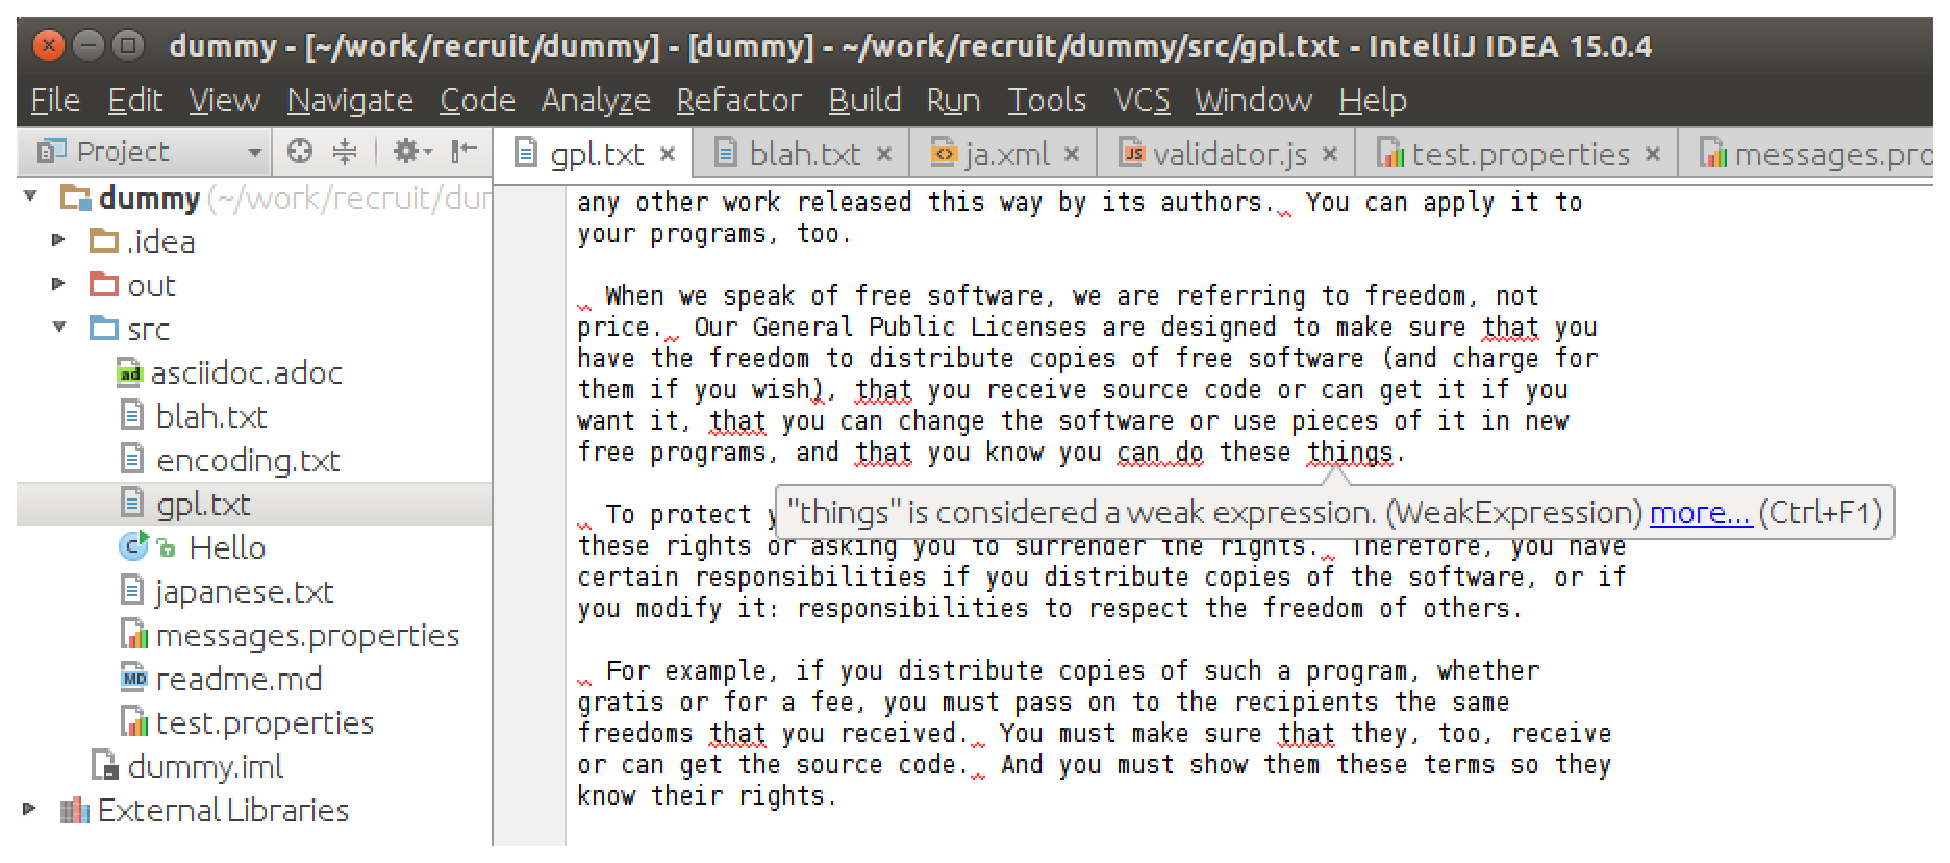
\includegraphics[width=8cm]{figs/intellij.eps}
  \end{center}
  \caption{IntelliJ IDEA の RedPen パッケージ}
  \label{fig:intellij-idea}
\end{figure}  

\section{RedPenの拡張}
\label{sec:extension}

RedPen は数十の文書検査用の機能を提供している。それでもユーザによっては必要な機能足りない場合がある。
そこで RedPen ユーザが機能を自作できる環境(プラグイン機構)を用意している。プラグインは Java と JavaScript で記述できる。
どちらで機能を作成しても問題ないが、JavaScript の方が手軽に作成できる。本節では JavaScript を利用した機能の作成方法をについて解説する。

機能を作成するには、validateSentence か validateSection 関数を実装する。
それぞれ、ドキュメント内に存在する全ての文もしくは節が引数として適用されます。今回はサンプルとして、長すぎる漢字列
を検知する機能を作成する。

\begin{figure}
  \scriptsize
  \small
  \begin{verbatim}
function validateSentence(sentence) {
    var pat = new RegExp("[\u4e00-\u9faf]{6,}", 'g');

    while (m = pat.exec(sentence.content)) {
      addError('長い熟語 "' + m[0] + '" (' +
              m[0].length + ') +
              が使われています。', sentence);
   }
}
  \end{verbatim}
  \normalsize
  \caption{長すぎる漢字列を検知する機能の実装例}
  \label{fig:js-validator}
\end{figure}

図~\ref{fig:js-validator} をみると、機能の実装は数行で実現できていることがわかる。
機能の作成では、まず漢字が6つ連続で出現するとマッチする正規表現を作成している。
その後、各文についてが正規表現とマッチするかを判定している。
正規表現にマッチするとエラーを addError 関数で作成~\footnote{addError関数は RedPen によって提供されている関数} している。

\section{まとめ}
本稿では自動ドキュメント検査ツール RedPen を解説した。その後、はじめにRedPenの特徴と、利用方法および拡張方法について紹介した。

\bibliographystyle{plain}
\bibliography{reference-j,reference}

\end{document}
